\documentclass{ximera}

%\usepackage{todonotes}

\newcommand{\todo}{}

\usepackage{tkz-euclide}
\tikzset{>=stealth} %% cool arrow head
\tikzset{shorten <>/.style={ shorten >=#1, shorten <=#1 } } %% allows shorter vectors

\usepackage{tkz-tab}  %% sign charts
\usetikzlibrary{decorations.pathreplacing} 

\usetikzlibrary{backgrounds} %% for boxes around graphs
\usetikzlibrary{shapes,positioning}  %% Clouds and stars
\usetikzlibrary{matrix} %% for matrix
\usepgfplotslibrary{polar} %% for polar plots
\usetkzobj{all}
\usepackage[makeroom]{cancel} %% for strike outs
%\usepackage{mathtools} %% for pretty underbrace % Breaks Ximera
\usepackage{multicol}

\usepackage{polynom}



\usepackage[many]{tcolorbox}  %% for titled boxes
\newtcolorbox{xbox}[1]{%
    tikznode boxed title,
    enhanced,
    arc=0mm,
    interior style={white},
    attach boxed title to top center= {yshift=-\tcboxedtitleheight/2},
    fonttitle=\bfseries,
    colbacktitle=white,coltitle=black,
    boxed title style={size=normal,colframe=white,boxrule=0pt},
    title={#1}}


\usepackage{array}
\setlength{\extrarowheight}{+.1cm}   
\newdimen\digitwidth
\settowidth\digitwidth{9}
\def\divrule#1#2{
\noalign{\moveright#1\digitwidth
\vbox{\hrule width#2\digitwidth}}}





\newcommand{\RR}{\mathbb R}
\newcommand{\R}{\mathbb R}
\newcommand{\N}{\mathbb N}
\newcommand{\Z}{\mathbb Z}

%\renewcommand{\d}{\,d\!}
\renewcommand{\d}{\mathop{}\!d}
\newcommand{\dd}[2][]{\frac{\d #1}{\d #2}}
\newcommand{\pp}[2][]{\frac{\partial #1}{\partial #2}}
\renewcommand{\l}{\ell}
\newcommand{\ddx}{\frac{d}{\d x}}
\newcommand{\ddt}{\frac{d}{\d t}}

\newcommand{\zeroOverZero}{\ensuremath{\boldsymbol{\tfrac{0}{0}}}}
\newcommand{\inftyOverInfty}{\ensuremath{\boldsymbol{\tfrac{\infty}{\infty}}}}
\newcommand{\zeroOverInfty}{\ensuremath{\boldsymbol{\tfrac{0}{\infty}}}}
\newcommand{\zeroTimesInfty}{\ensuremath{\small\boldsymbol{0\cdot \infty}}}
\newcommand{\inftyMinusInfty}{\ensuremath{\small\boldsymbol{\infty - \infty}}}
\newcommand{\oneToInfty}{\ensuremath{\boldsymbol{1^\infty}}}
\newcommand{\zeroToZero}{\ensuremath{\boldsymbol{0^0}}}
\newcommand{\inftyToZero}{\ensuremath{\boldsymbol{\infty^0}}}



\newcommand{\numOverZero}{\ensuremath{\boldsymbol{\tfrac{\#}{0}}}}
\newcommand{\dfn}{\textbf}
%\newcommand{\unit}{\,\mathrm}
\newcommand{\unit}{\mathop{}\!\mathrm}
\newcommand{\eval}[1]{\bigg[ #1 \bigg]}
\newcommand{\seq}[1]{\left( #1 \right)}
\renewcommand{\epsilon}{\varepsilon}
\renewcommand{\iff}{\Leftrightarrow}

\DeclareMathOperator{\arccot}{arccot}
\DeclareMathOperator{\arcsec}{arcsec}
\DeclareMathOperator{\arccsc}{arccsc}
\DeclareMathOperator{\si}{Si}
\DeclareMathOperator{\proj}{proj}
\DeclareMathOperator{\scal}{scal}


\newcommand{\tightoverset}[2]{% for arrow vec
  \mathop{#2}\limits^{\vbox to -.5ex{\kern-0.75ex\hbox{$#1$}\vss}}}
\newcommand{\arrowvec}[1]{\tightoverset{\scriptstyle\rightharpoonup}{#1}}
\renewcommand{\vec}{\mathbf}
\newcommand{\veci}{\vec{i}}
\newcommand{\vecj}{\vec{j}}
\newcommand{\veck}{\vec{k}}
\newcommand{\vecl}{\boldsymbol{\l}}

\newcommand{\dotp}{\bullet}
\newcommand{\cross}{\boldsymbol\times}
\newcommand{\grad}{\boldsymbol\nabla}
\newcommand{\divergence}{\grad\dotp}
\newcommand{\curl}{\grad\cross}
%\DeclareMathOperator{\divergence}{divergence}
%\DeclareMathOperator{\curl}[1]{\grad\cross #1}


\colorlet{textColor}{black} 
\colorlet{background}{white}
\colorlet{penColor}{blue!50!black} % Color of a curve in a plot
\colorlet{penColor2}{red!50!black}% Color of a curve in a plot
\colorlet{penColor3}{red!50!blue} % Color of a curve in a plot
\colorlet{penColor4}{green!50!black} % Color of a curve in a plot
\colorlet{penColor5}{orange!80!black} % Color of a curve in a plot
\colorlet{fill1}{penColor!20} % Color of fill in a plot
\colorlet{fill2}{penColor2!20} % Color of fill in a plot
\colorlet{fillp}{fill1} % Color of positive area
\colorlet{filln}{penColor2!20} % Color of negative area
\colorlet{fill3}{penColor3!20} % Fill
\colorlet{fill4}{penColor4!20} % Fill
\colorlet{fill5}{penColor5!20} % Fill
\colorlet{gridColor}{gray!50} % Color of grid in a plot

\newcommand{\surfaceColor}{violet}
\newcommand{\surfaceColorTwo}{redyellow}
\newcommand{\sliceColor}{greenyellow}




\pgfmathdeclarefunction{gauss}{2}{% gives gaussian
  \pgfmathparse{1/(#2*sqrt(2*pi))*exp(-((x-#1)^2)/(2*#2^2))}%
}


%%%%%%%%%%%%%
%% Vectors
%%%%%%%%%%%%%

%% Simple horiz vectors
\renewcommand{\vector}[1]{\left\langle #1\right\rangle}


%% %% Complex Horiz Vectors with angle brackets
%% \makeatletter
%% \renewcommand{\vector}[2][ , ]{\left\langle%
%%   \def\nextitem{\def\nextitem{#1}}%
%%   \@for \el:=#2\do{\nextitem\el}\right\rangle%
%% }
%% \makeatother

%% %% Vertical Vectors
%% \def\vector#1{\begin{bmatrix}\vecListA#1,,\end{bmatrix}}
%% \def\vecListA#1,{\if,#1,\else #1\cr \expandafter \vecListA \fi}

%%%%%%%%%%%%%
%% End of vectors
%%%%%%%%%%%%%

%\newcommand{\fullwidth}{}
%\newcommand{\normalwidth}{}



%% makes a snazzy t-chart for evaluating functions
%\newenvironment{tchart}{\rowcolors{2}{}{background!90!textColor}\array}{\endarray}

%%This is to help with formatting on future title pages.
\newenvironment{sectionOutcomes}{}{} 



%% Flowchart stuff
%\tikzstyle{startstop} = [rectangle, rounded corners, minimum width=3cm, minimum height=1cm,text centered, draw=black]
%\tikzstyle{question} = [rectangle, minimum width=3cm, minimum height=1cm, text centered, draw=black]
%\tikzstyle{decision} = [trapezium, trapezium left angle=70, trapezium right angle=110, minimum width=3cm, minimum height=1cm, text centered, draw=black]
%\tikzstyle{question} = [rectangle, rounded corners, minimum width=3cm, minimum height=1cm,text centered, draw=black]
%\tikzstyle{process} = [rectangle, minimum width=3cm, minimum height=1cm, text centered, draw=black]
%\tikzstyle{decision} = [trapezium, trapezium left angle=70, trapezium right angle=110, minimum width=3cm, minimum height=1cm, text centered, draw=black]


\title[Dig-In:]{Exponential and logarithmetic functions}


\begin{document}
\begin{abstract}
  Exponential and logarithmic functions illuminated.
\end{abstract}
\maketitle

Exponential and logarithmic functions may seem somewhat esoteric at
first, but they model many phenomena in the real-world.




\section{What are exponential and logarithmic functions?}


\begin{definition}
  An \dfn{exponential function} is a function of the form
  \[
  f(x) = b^x
  \]
  where  $b\ne 1$ is a positive real number. The domain of an
  exponential function is $(-\infty,\infty)$ and the range is $(0, \infty)$.
\end{definition}

\begin{question}
  Is $b^{-x}$ an exponential function?
  \begin{multipleChoice}
    \choice[correct]{yes}
    \choice{no}
  \end{multipleChoice}
  \begin{feedback}
    Note that
    \[
    b^{-x} = \left(b^{-1}\right)^x = \left(\frac{1}{b}\right)^x.
    \]
  \end{feedback}
\end{question}


\begin{definition}
  A \dfn{logarithmic function} is a function defined as follows
  \[
  \log_b(x) = y \qquad\text{means that}\qquad b^y = x
  \]
  where  $b\ne 1$ is a positive real number. The domain of a
  logarithmic function is $(0,\infty)$ and the range is $(- \infty, \infty)$.
\end{definition}

In either definition above $b$ is called the \dfn{base}.

Remember that with exponential and logarithmic functions, there is one very special
base:
\[ e = 2.7182818284590\ldots \]
This is an irrational number that you will see frequently.  The exponential with base $e$,
$f(x) = e^x$ is often called the `natural exponential' function.  For the logarithm with base $e$,
we have a special notation, $\ln x$ is `natural logarithm' function.   We'll talk about where $e$
comes from when we talk about derivatives.


\subsection{Connections between exponential functions and logarithms}

Let $b$ be a positive real number with $b\ne 1$.
\begin{itemize}
\item $b^{\log_b(x)} = x$ for all positive $x$
\item $\log_b(b^x) = x$ for all real $x$
\end{itemize}

\begin{question}
  What exponent makes the following expression true?
  \[
  3^x = e^{\left( x \cdot \answer{\ln 3} \right)}.
  \]
\end{question}


\section{What can the graphs look like?}

\subsection{Graphs of exponential functions}

\begin{example}
  Here we see the the graphs of four exponential functions.
  \begin{image}
    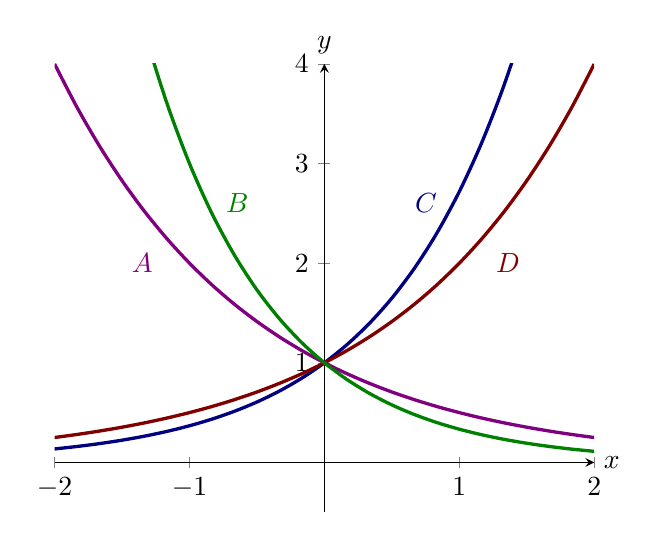
\begin{tikzpicture}
      \begin{axis}[
          domain=-2:2,
          xmin=-2, xmax=2,
          ymin=-.5, ymax=4,
          axis lines =middle, xlabel=$x$, ylabel=$y$,
          every axis y label/.style={at=(current axis.above origin),anchor=south},
          every axis x label/.style={at=(current axis.right of origin),anchor=west},
        ]
	\addplot [very thick, penColor, smooth] {e^x};
        \addplot [very thick, penColor2, smooth] {2^x)};
        \addplot [very thick, penColor3, smooth] {(1/2)^x)};
        \addplot [very thick, penColor4, smooth] {(1/3)^x)};
        
        
        
        \node at (axis cs:-1.5, 2 ) [penColor3,anchor=west] {$A$};
        \node at (axis cs:-.8, 2.6 ) [penColor4,anchor=west] {$B$};
        \node at (axis cs:0.6, 2.6 ) [penColor,anchor=west] {$C$};
        \node at (axis cs:1.2, 2 ) [penColor2,anchor=west] {$D$};
        
      \end{axis}
    \end{tikzpicture}
  \end{image}
  Match the curves $A$, $B$, $C$, and $D$ with the functions
  \[
  e^x, \qquad \left(\frac{1}{2}\right)^{x}, \qquad  \left(\frac{1}{3}\right)^{x}, \qquad 2^{x}.
  \]
  \begin{explanation}
    One way to solve these problems is to compare these functions
    along the vertical line $x=1$,
    \begin{image}
      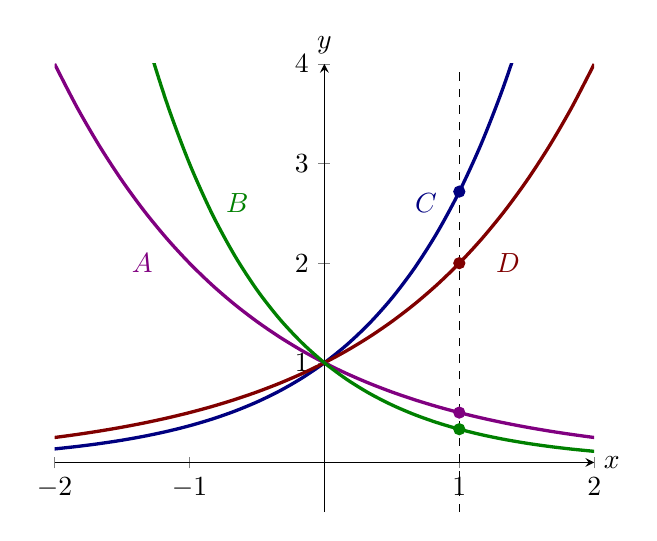
\begin{tikzpicture}
        \begin{axis}[
            domain=-2:2,
            xmin=-2, xmax=2,
            ymin=-.5, ymax=4,
            axis lines =middle, xlabel=$x$, ylabel=$y$,
            every axis y label/.style={at=(current axis.above origin),anchor=south},
            every axis x label/.style={at=(current axis.right of origin),anchor=west},
          ]
	  \addplot [very thick, penColor, smooth] {e^x}; %C
          \addplot [very thick, penColor2, smooth] {2^x)};%D
          \addplot [very thick, penColor3, smooth] {(1/2)^x)};%A
          \addplot [very thick, penColor4, smooth] {(1/3)^x)};%B
            
          \node at (axis cs:-1.5, 2 ) [penColor3,anchor=west] {$A$};
          \node at (axis cs:-.8, 2.6 ) [penColor4,anchor=west] {$B$};
          \node at (axis cs:0.6, 2.6 ) [penColor,anchor=west] {$C$};
          \node at (axis cs:1.2, 2 ) [penColor2,anchor=west] {$D$};

          \addplot [textColor, dashed] plot coordinates {(1,-.5) (1,4)};

          \addplot[color=penColor,fill=penColor,only marks,mark=*] coordinates{(1,e)}; %C
          \addplot[color=penColor2,fill=penColor2,only marks,mark=*] coordinates{(1,2)}; %D
          \addplot[color=penColor3,fill=penColor3,only marks,mark=*] coordinates{(1,1/2)}; %A
          \addplot[color=penColor4,fill=penColor4,only marks,mark=*] coordinates{(1,1/3)}; %B
        \end{axis}
      \end{tikzpicture}
    \end{image}
    Note
    \[
    \left(\frac{1}{3}\right)^1 < \left(\frac{1}{2}\right)^1  < 2^1 < e^1.
    \]
    Hence we see:
    \begin{itemize}
    \item $\left(\frac{1}{3}\right)^{x}$ corresponds to
      $\answer[given]{B}$.
    \item $\left(\frac{1}{2}\right)^{x}$ corresponds to $\answer[given]{A}$.
    \item $2^x$ corresponds to $\answer[given]{D}$.
    \item $e^x$ corresponds to $\answer[given]{C}$.
    \end{itemize}
  \end{explanation}
\end{example}



\subsection{Graphs of logarithmic functions}


\begin{example}
  Here we see the the graphs of four logarithmic functions.
  \begin{image}
    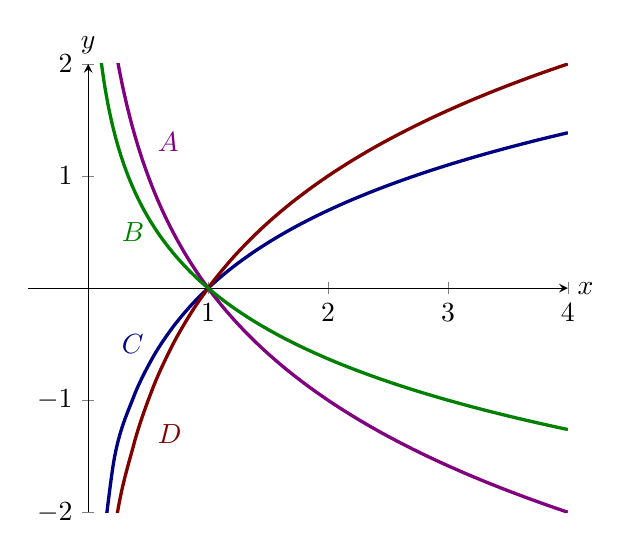
\begin{tikzpicture}
      \begin{axis}[
          domain=0.05:4,
          xmin=-.5, xmax=4,
          ymin=-2, ymax=2,
          axis lines =middle, xlabel=$x$, ylabel=$y$,
          every axis y label/.style={at=(current axis.above origin),anchor=south},
          every axis x label/.style={at=(current axis.right of origin),anchor=west},
        ]
	\addplot [very thick, penColor, smooth] {ln(x)}; % C
        \addplot [very thick, penColor2, smooth] {ln(x)/ln(2)}; % D
        \addplot [very thick, penColor3, smooth, samples=100] {ln(x)/ln(1/2))}; % A
        \addplot [very thick, penColor4, smooth, samples=100] {ln(x)/ln(1/3))}; %B
        
        
        \node at (axis cs:.5, 1.3 ) [penColor3,anchor=west] {$A$};
        \node at (axis cs:.2, .5 ) [penColor4,anchor=west] {$B$};
        \node at (axis cs:0.2, -.5 ) [penColor,anchor=west] {$C$};
        \node at (axis cs:.5, -1.3 ) [penColor2,anchor=west] {$D$};
        
      \end{axis}
    \end{tikzpicture}
  \end{image}
  Match the curves $A$, $B$, $C$, and $D$ with the functions
  \[
  \ln(x),\qquad \log_{1/2}(x), \qquad \log_{1/3}(x),\qquad \log_2(x).
  \]
  \begin{explanation}
    First remember what $\log_b(x)=y$ means:
    \[
    \log_b(x) = y \qquad\text{means that}\qquad b^y = x.
    \]
    Moreover, $\ln(x) = \log_e(x)$ where $e= 2.71828\dots$.  So now
    examine each of these functions along the horizontal line $y=1$
    \begin{image}
      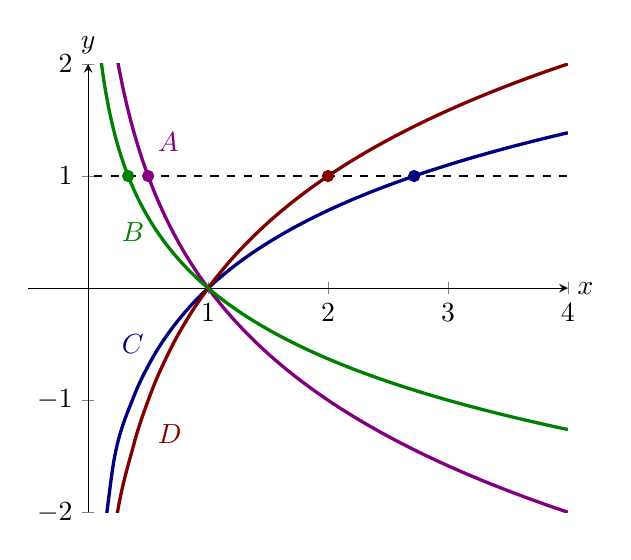
\begin{tikzpicture}
        \begin{axis}[
            domain=0.05:4,
            xmin=-.5, xmax=4,
            ymin=-2, ymax=2,
            axis lines =middle, xlabel=$x$, ylabel=$y$,
            every axis y label/.style={at=(current axis.above origin),anchor=south},
            every axis x label/.style={at=(current axis.right of origin),anchor=west},
          ]
	  \addplot [very thick, penColor, smooth] {ln(x)}; % C
          \addplot [very thick, penColor2, smooth] {ln(x)/ln(2)}; % D
          \addplot [very thick, penColor3, smooth, samples=100] {ln(x)/ln(1/2))}; % A
          \addplot [very thick, penColor4, smooth, samples=100] {ln(x)/ln(1/3))}; %B
          \addplot [dashed] {1};
        
          
          \node at (axis cs:.5, 1.3 ) [penColor3,anchor=west] {$A$};
          \node at (axis cs:.2, .5 ) [penColor4,anchor=west] {$B$};
          \node at (axis cs:0.2, -.5 ) [penColor,anchor=west] {$C$};
          \node at (axis cs:.5, -1.3 ) [penColor2,anchor=west] {$D$};

          \addplot[color=penColor,fill=penColor,only marks,mark=*] coordinates{(e,1)}; %C
          \addplot[color=penColor2,fill=penColor2,only marks,mark=*] coordinates{(2,1)}; %D
          \addplot[color=penColor3,fill=penColor3,only marks,mark=*] coordinates{(1/2,1)}; %A
          \addplot[color=penColor4,fill=penColor4,only marks,mark=*] coordinates{(1/3,1)}; %B
        \end{axis}
      \end{tikzpicture}
    \end{image}
    Note again (this is from the definition of a logarithm)
    \[
    \left(\frac{1}{3}\right)^1 < \left(\frac{1}{2}\right)^1  < 2^1 < e^1.
    \]
    Hence we see:
    \begin{itemize}
    \item $\log_{1/3}(x)$ corresponds to $\answer[given]{B}$.
    \item $\log_{1/2}(x)$ corresponds to $\answer[given]{A}$.
    \item $\log_2(x)$ corresponds to $\answer[given]{D}$.
    \item $\ln(x)$ corresponds to $\answer[given]{C}$.
    \end{itemize}
  \end{explanation}
\end{example}



\section{Properties of exponential functions and logarithms}

Working with exponential and logarithmic functions is often simplified by  
applying properties of these functions.  These properties will make appearances 
throughout our work.

\subsection{Properties of exponents}
Let $b$ be a positive real number with $b\ne 1$.
\begin{itemize}
  \item $b^m\cdot b^n = b^{m+n}$
  \item $b^{-1} = \frac{1}{b}$
  \item $\left(b^m\right)^n = b^{mn}$
\end{itemize}
\begin{question}
  What exponent makes the following true?
  \[
  2^4 \cdot 2^3 = 2^{\answer{7}}
  \]
  \begin{hint}
    \[
    (2^4) \cdot (2^3) = (2 \cdot 2\cdot 2 \cdot 2) \cdot  (2 \cdot 2\cdot 2)
    \]
  \end{hint}
\end{question}

\subsection{Properties of logarithms}
Let $b$ be a positive real number with $b\ne 1$.
\begin{itemize}
\item $\log_b(m\cdot n) = \log_b(m) + \log_b(n)$
\item $\log_b(m^n) = n\cdot \log_b(m)$
\item $\log_b\left(\frac{1}{m}\right) = \log_b(m^{-1}) = -\log_b(m)$
\item $\log_a(m) = \frac{\log_b(m)}{\log_b(a)}$
\end{itemize}

\begin{question}
  What value makes the following expression true?
  \[
  \log_2\left(\frac{8}{16}\right) = 3-\answer{4}
  \]
\end{question}


\begin{question}
  What makes the following expression true?
  \[
  \log_3(x) = \frac{\ln(x)}{\answer{\ln(3)}}
  \]
\end{question}


\section{Exponential equations}
Let's look into solving equations involving these functions.  We'll start with a straightforward example.
\begin{example}
	Solve the equation: $\displaystyle 4^x = 8$.
	\begin{explanation}
		We know $4$ and $8$ are each powers of $2$, we start by rewriting in terms of this base.
		\[ 4^x = 2^{2x}  \,\,\, \textrm{ and } \,\,\, 8 =2^{\answer{3}} \,\,\,\, \textrm{ so } 2^{2x} = 2^{\answer{3}} \]
		Since exponential functions are one-to-one, the only way for $a^m = a^n$ is if $m=n$.  In this case,
		that means $\displaystyle 2x = 3$.
		
		The solution is: $\displaystyle x = \answer{3/2}$.
	\end{explanation}
\end{example}


Of course, if we couldn't rewrite both sides with the same base, we can still use the properties of logarithms to solve.
\begin{example}
	Solve the equation: $\displaystyle 5^{2x-3} = 7$.
	\begin{explanation}
		Since we can't easily rewrite both sides as exponentials with the same base, we'll use logarithms instead.  Above we said that
		$\log_b(x) = y$ means that $b^y = x$.  That statement means that each exponential equation has an equivalent logarithmic form
		and vice-versa.  We'll convert to a logarithmic equation and solve from there.
		\begin{align*}
			5^{2x-3} &= 7\\
			\log_{\answer{5}}\left(  \answer{7} \right) &= 2x-3
		\end{align*}
		From here, we can solve for $x$ directly.
		\begin{align*}
			2x &= \log_{5}\left(7\right) + 3\\
			x &= \frac{\log_{5}\left(7\right) + 3}{2}
		\end{align*}
	\end{explanation} 
\end{example}


\begin{example}
	Solve the equation: $\displaystyle e^{2x} = e^x + 6$. 
	\begin{explanation}
		Immediately taking logarithms of both sides will not help here, as the right side has multiple terms.  We know that logarithms do not
		behave well with sums, but with products/quotients.  Instead, we notice that $e^{2x} = \left(e^x\right)^2$. (This is a common trick that
		you will likely see many times.)  
		\begin{align*}
			e^{2x} &= e^x + 6\\
			\left(e^x\right)^2 &= e^x + 6\\
			\left(e^x\right)^2 - e^x - 6 &= 0
		\end{align*}
		Our equation is really a quadratic equation in $e^x$!  The left-hand side factors as $\left( e^x - \answer{3}\right) \left(e^x + \answer{2}\right)$, so we are dealing
		with \[ e^x - \answer{3} = 0  \qquad  \textrm{and} \qquad e^x+\answer{2} = 0.\]
		For the first:
		\begin{align*}
			e^x &= \answer{3}\\
			x &= \ln\left( \answer{3}\right).
		\end{align*}
		
		From the second: $\displaystyle e^x = \answer{-2}$.  Look back at the graph of $y=e^x$ above.  What was the range of the exponential function?  It didn't include any negative
		numbers, so $e^x = -2$ has no solutions. 
		
		The solution to $\displaystyle e^{2x} = e^x + 6$ is $x = \answer{\ln(3)}$.
	\end{explanation}
\end{example}

\begin{problem}
	Solve the equation: $\displaystyle 2\left(5^{2x} + 6\right) = 11 \cdot 5^x$.
	\begin{selectAll}
		\choice[correct]{$\displaystyle \log_{5}\left(\dfrac{3}{2} \right)$}
		\choice{$\displaystyle \frac{\ln\left(\dfrac{3}{2} \right)}{5}$}
		\choice{$\displaystyle \log_{4}\left(5\right)$}
		\choice[correct]{$\displaystyle \log_{5}\left(4 \right)$}
		\choice{The equation has no solutions.}
	\end{selectAll}
\end{problem}

\begin{example}
	Solve the inequality: $\displaystyle \frac{6^x - 7 \cdot 3^x}{4^x - 15} \ge 0$.
	\begin{explanation}
		Since this isn't a linear inequality, we'll solve it using a sign-chart.  Luckily, the right-side is already $0$.  Let's factor the numerator on the left:
		\begin{align*} 
			6^x - 7 \cdot 3^x &= \left(2\cdot 3\right)^x - 7 \cdot 3^x \\
				&= 2^x \cdot 3^x - 7 \cdot 3^x\\
				&= 3^x \left( 2^x - 7 \right).
		\end{align*}
		That means we need to construct a sign chart for $\displaystyle \frac{3^x \left( 2^x - 7\right)}{4^x - 15}$.
		(Note: $\log_{2}(7)$ is about $2.81$ and $\log_{4}(15)$ is about $1.95$.)
		
		\begin{center}
		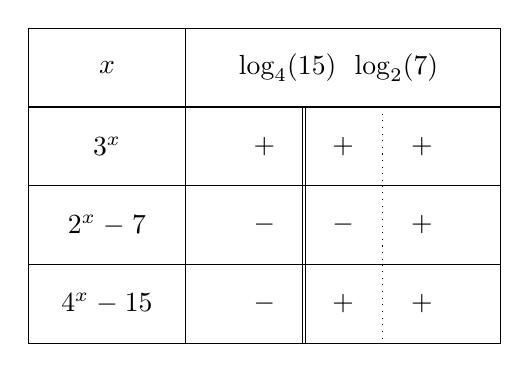
\begin{tikzpicture} 
			\tkzTabInit[lgt=2,espcl=1] 
				{$x$         /1, 
				$3^x$   /1, 
				$2^x-7$  /1,
				$4^x-15$       /1}% 
				{  , $\log_{4}(15)$ \,\,\,\,\, , \,\,\,\,\,\,$\log_{2}(7)$ ,  }% 
			\tkzTabLine{ , + , d , +  , t , + ,}
			\tkzTabLine{ , - , d , - , t , + ,}
			\tkzTabLine{ , - , d ,  + , t , +, }
		\end{tikzpicture} 
		\end{center}
		The solution is:
		\[ \left( -\infty, \, \log_{4}(15) \, \right) \bigcup \left[ \,\log_{2}(7) \,, \infty \right) \]
	\end{explanation}
\end{example}
\section{Logarithmic equations}

\begin{example}
	Solve the equation: $\displaystyle \log_5( 2x+1) = 3$.
	\begin{explanation}
		Our first step will be to rewrite this logarithmic equation into its exponential form.
		\[ \log_5(2x+1) = 3 \qquad \textrm{ means } \qquad 2x+1 = 5^{\answer{3}} \]
		From here we solve directly.
		\begin{align*}
			2x+1 &= \answer{125}\\
			2x &= \answer{124}\\
			x &= \answer{62}.
		\end{align*}
	\end{explanation}
\end{example}



\begin{example}
	Solve the equation: \[ \log_3(2x+1) = 1-\log_3(x+2). \]
	\begin{explanation}
		With more than one logarithm, we'll typically try to use the properties of logarithms to combine them into a single term.
		\begin{align*}
			\log_3(2x+1) &= 1-\log_3(x+2) \\
			\log_3(2x+1) + \log_3(x+2) &= 1\\
			\log_3\left( (2x+1)(x+2)\right) &= 1\\
			\log_3\left( 2x^2 + 5x + 2 \right) &= 1\\
			2x^2 + 5x + 2 &= 3\\
			2x^2 + 5x - 1 &= 0
		\end{align*}
		Let's use quadratic formula to solve this.
		\[ x = \frac{-5 \pm \sqrt{5^2 - 4 \cdot 2\cdot -1}}{2 \cdot 2} = \frac{ -5\pm \sqrt{ \answer{33} } }{4}. \]
		
		What happens if we try to plug $x = \dfrac{-5 - \sqrt{33}}{4}$ into the equation?  Both $2\left( \dfrac{-5-\sqrt{33}}{4} \right) + 1$ and $\dfrac{-5-\sqrt{33}}{4} + 2$ are 
		negative.  That means, the logarithms of these values is not defined.  
		
		It turns out that $\dfrac{-5 - \sqrt{33}}{4}$ is a solution of the equation $2x^2+5x-1 = 0$,
		but not a solution of the original equation $\log_3(2x+1) = 1-\log_3(x+2)$. 
		
		When working with logarithmic equations, we must always check that the solutions we find 
		actually satisfy the original equation.
		
		The only solution is $x = \dfrac{-5 + \sqrt{33}}{4}$.
		
	\end{explanation}		
\end{example}





\end{document}
